\documentclass[xcolor=dvipsnames]{beamer}

% For more themes, color themes and font themes, see:
% http://deic.uab.es/~iblanes/beamer_gallery/index_by_theme.html

\mode<presentation>
{
  \usetheme{Boadilla}      
  \usecolortheme{default} 
  \usefonttheme{default} 
  \setbeamertemplate{navigation symbols}{}
  \setbeamertemplate{caption}[numbered]
} 

\usepackage[english]{babel}
\usepackage[utf8x]{inputenc}

\usepackage{xcolor}
\usepackage{color}
\definecolor{rscuro}{rgb}{0.75,0.0,0.0}
\definecolor{bscuro}{rgb}{0.0,0.2,0.5}

\usepackage{graphicx}
\graphicspath{{Presentation_images/}}                 								
\usepackage[font=small,format=hang]{caption}  										
\captionsetup{tableposition=top,figureposition=bottom,font=small, format=hang,labelfont={sf,bf}} 	
\usepackage{subfig}

\usepackage{eurosym}

\title[Topics in Statistical learning]{}
\author{L. Insolia, J. Kim and Y. Yeghikyan}
\institute{SNS}
\date{March 9, 2018}

\begin{document}
	
	\begin{frame}
		\vskip 1.5cm 	
 		\centering\huge\textcolor{bscuro}{Study of French labour market and inequalities} \\
		\vskip 0.5cm 
			\centering\small \textcolor{rscuro}{--- \emph{Midterm results} ---}
			\maketitle
	\end{frame}
	
	%\begin{frame}{Outline}
	%\tableofcontents
	%\end{frame}
	
	
\section{Motivation}
		\begin{frame}{\vskip 0.05cm\centerline{\Huge\textcolor{bscuro}{Objectives}}}
%	   What were the aims of your project, and what is the context – in terms of subject matter questions, and in terms of applicable statistical and computational tools.  		
			
			\begin{itemize}
			 	 \item Structure of French labour market 
			 	 \item Inequalities (in terms of salary): 
			 	 \begin{itemize}
			 	 	\item ages 
			 	 	\item gender
			 	 	\item job categories
			 	 	\item spatial distribution
			 	 \end{itemize}
		 	 	 \item Firms' distribution
		 	 	 \item Exploratory analyses
			\end{itemize}
			\vskip 1cm
\end{frame}
	
	
\section{Methodology}
		\begin{frame}{\vskip 0.05cm\centerline{\Huge\textcolor{bscuro}{Methodology}}}
%	  Description of the dataset (where is it from what is the information shared through this dataset, what year)and the variables that we have, what are the interesting features that we can use to study 
% 		\begin{itemize}
		INSEE data
				\begin{itemize}
				\item Population: age, sex and cohabitation mode
				\item Salary: job categories, age and sex (mean net salary per hour in \euro)
				\item Firms: number of firms for each size
				\item Geography: GPS location
				\end{itemize}
		for different geographical levels (communes, departments, \underline{towns}) in 2014
%		\end{itemize}				
\end{frame}
	
	
\section{1. What has been done so far...}
		\begin{frame}%{\vskip 0.05cm\centerline{\Huge\textcolor{bscuro}{What has been done so far \ldots}}}
%	  State clearly what you were able to accomplish during the course, illustrate methods used and results.
		\vskip 1.8cm \centerline{\Huge\textcolor{bscuro}{What has been done so far \ldots}}

\end{frame}


\section{1. Graphes}
		\begin{frame}{\centerline{\huge\textcolor{bscuro}{Population}}}

		\begin{itemize}
			\item Created new features 
			\item Insights to demographic profile 
		\end{itemize}
%		\begin{itemize}
%			\item insight to demographic profile for each town 
%			\item age into three different categories: child, workforce and elderly
%			\item sex and dependency ratios 
%		\end{itemize}
%		Fig.~\ref{fig1} shows 
			\begin{figure}[!ht] 
				\centering
				\subfloat{{\includegraphics[width=5.5cm]{dis_pop_dep.jpeg} }}
%				\qquad
				\subfloat{{\includegraphics[width=5.5cm]{pyramid_pop.jpeg} }}
%				\*caption{111} 
%				\label{fig1}
			\end{figure}
		\end{frame}


%\section{2. What has been done so far...}
%\begin{frame}{\vskip 0.05cm\centerline{\Huge\textcolor{bscuro}{What has been done so far \ldots}}}
%%	  State clearly what you were able to accomplish during the course, illustrate methods used and results.
%\begin{itemize}
%	\item Salary:
%	\begin{itemize}
%		\item salary levels across different towns
%		\item comparison for different job positions, genders, ages
%		\item predictions of 
%	\end{itemize}
%\end{itemize}
%\end{frame}


\section{2. Graphes}

	\begin{frame}{\centerline{\huge\textcolor{bscuro}{Salary}}}
%		Fig.~\ref{fig2} shows 
		
		\begin{itemize}
			\item Inequality of salary
		\end{itemize}
	
\begin{figure}[!ht] 
	\centering
	\subfloat{\includegraphics[width=0.5\textwidth]{boxplot_sex_age.jpeg}} 
	\subfloat{\includegraphics[width=0.5\textwidth]{boxplot_sex_job.jpeg}}
	%			\caption{} 
	%			\label{fi	g2}
\end{figure}
\end{frame}


	\begin{frame}{\centerline{\huge\textcolor{bscuro}{Salary}}}
%		Fig.~\ref{fig2} shows 

		\begin{figure}[!ht] 
			\centering
			\subfloat{\includegraphics[width=0.5\textwidth]{hist_salary_ratio_general.jpeg}} 
			\subfloat{\includegraphics[width=0.5\textwidth]{scatter_salary_ratio_vs_general.jpeg}}
%			\caption{} 
%			\label{fi	g2}
		\end{figure}
\end{frame}


\section{2.1 Graphes} 
\begin{frame}{\centerline{\huge\textcolor{bscuro}{Salary}}}
%Fig.~\ref{fig3} shows 
		\begin{figure}[!ht] 
	\centering
	\subfloat{\includegraphics[width=0.5\textwidth]{hist_salary_ratio_executives.jpeg}} 
	\subfloat{\includegraphics[width=0.5\textwidth]{hist_salary_ratioExec_vs_executives.jpeg}}
	%			\caption{} 
	%			\label{fi	g2}
\end{figure}
\end{frame}

\begin{frame}{\centerline{\huge\textcolor{bscuro}{Salary}}}
%Fig.~\ref{fig3} shows 
\begin{itemize}
	\item ANOVA using sex, job, age and interaction effects
\end{itemize}

\begin{figure}[!ht] 
	\centering
	\subfloat{\includegraphics[width=0.5\textwidth]{ANOVA_factors.jpeg}} 
	\subfloat{\includegraphics[width=0.5\textwidth]{ANOVA_model.jpeg}}
	%			\caption{} 
	%			\label{fi	g2}
\end{figure}
\end{frame} 

\begin{frame}{\centerline{\huge\textcolor{bscuro}{Salary}}}
\begin{figure}[!ht] 
	\centering
	\subfloat{\includegraphics[width=0.75\textwidth]{ANOVA_dataY.jpeg}} 
	%			\caption{} 
	%			\label{fi	g2}
\end{figure}
\end{frame}

\begin{frame}{\centerline{\huge\textcolor{bscuro}{Salary}}}
%Fig.~\ref{fig3} shows 
\begin{itemize}
	\item Prediction for young people using BSS 
\end{itemize}

\begin{figure}[!ht] 
	\centering
	\subfloat{\includegraphics[width=0.6\textwidth]{bestsubsel_18_25.jpeg}} 
	\qquad
	\subfloat{\includegraphics[width=0.5\textwidth]{bestsubsel_18_25_BIC.jpeg}}
	%			\caption{} 
	%			\label{fi	g2}
\end{figure}
\end{frame}

\begin{frame}{\centerline{\huge\textcolor{bscuro}{Salary}}}
%Fig.~\ref{fig3} shows 
\begin{itemize}
	\item Prediction for young people using elastic net and and 10-folds CV
\end{itemize}

\begin{figure}[!ht] 
	\centering
	\subfloat{\includegraphics[width=0.9\textwidth]{elasticNet_10foldsCV.jpeg}} 
%	\subfloat{\includegraphics[width=0.5\textwidth]{ANOVA_model.jpeg}}
	%			\caption{} 
	%			\label{fi	g2}
\end{figure}
\end{frame}

%\section{3. What has been done so far...}
%\begin{frame}{\centerline{\huge\textcolor{bscuro}{Firms}}}
%%	  State clearly what you were able to accomplish during the course, illustrate methods used and results.
%%\begin{itemize}
%%	\item Firms:
%%	\begin{itemize}
%%		\item distribution of firms per town
%%		\item analysis
%%	\end{itemize}
%%\end{itemize}
%\end{frame}



\section{3. Graphes}
	\begin{frame}{\centerline{\huge\textcolor{bscuro}{Firms}}}
%			Fig.~\ref{} shows 
\begin{itemize}
		\item Distribution of firms per town
\end{itemize}
			\begin{figure}[!ht] 
				\centering
				\subfloat{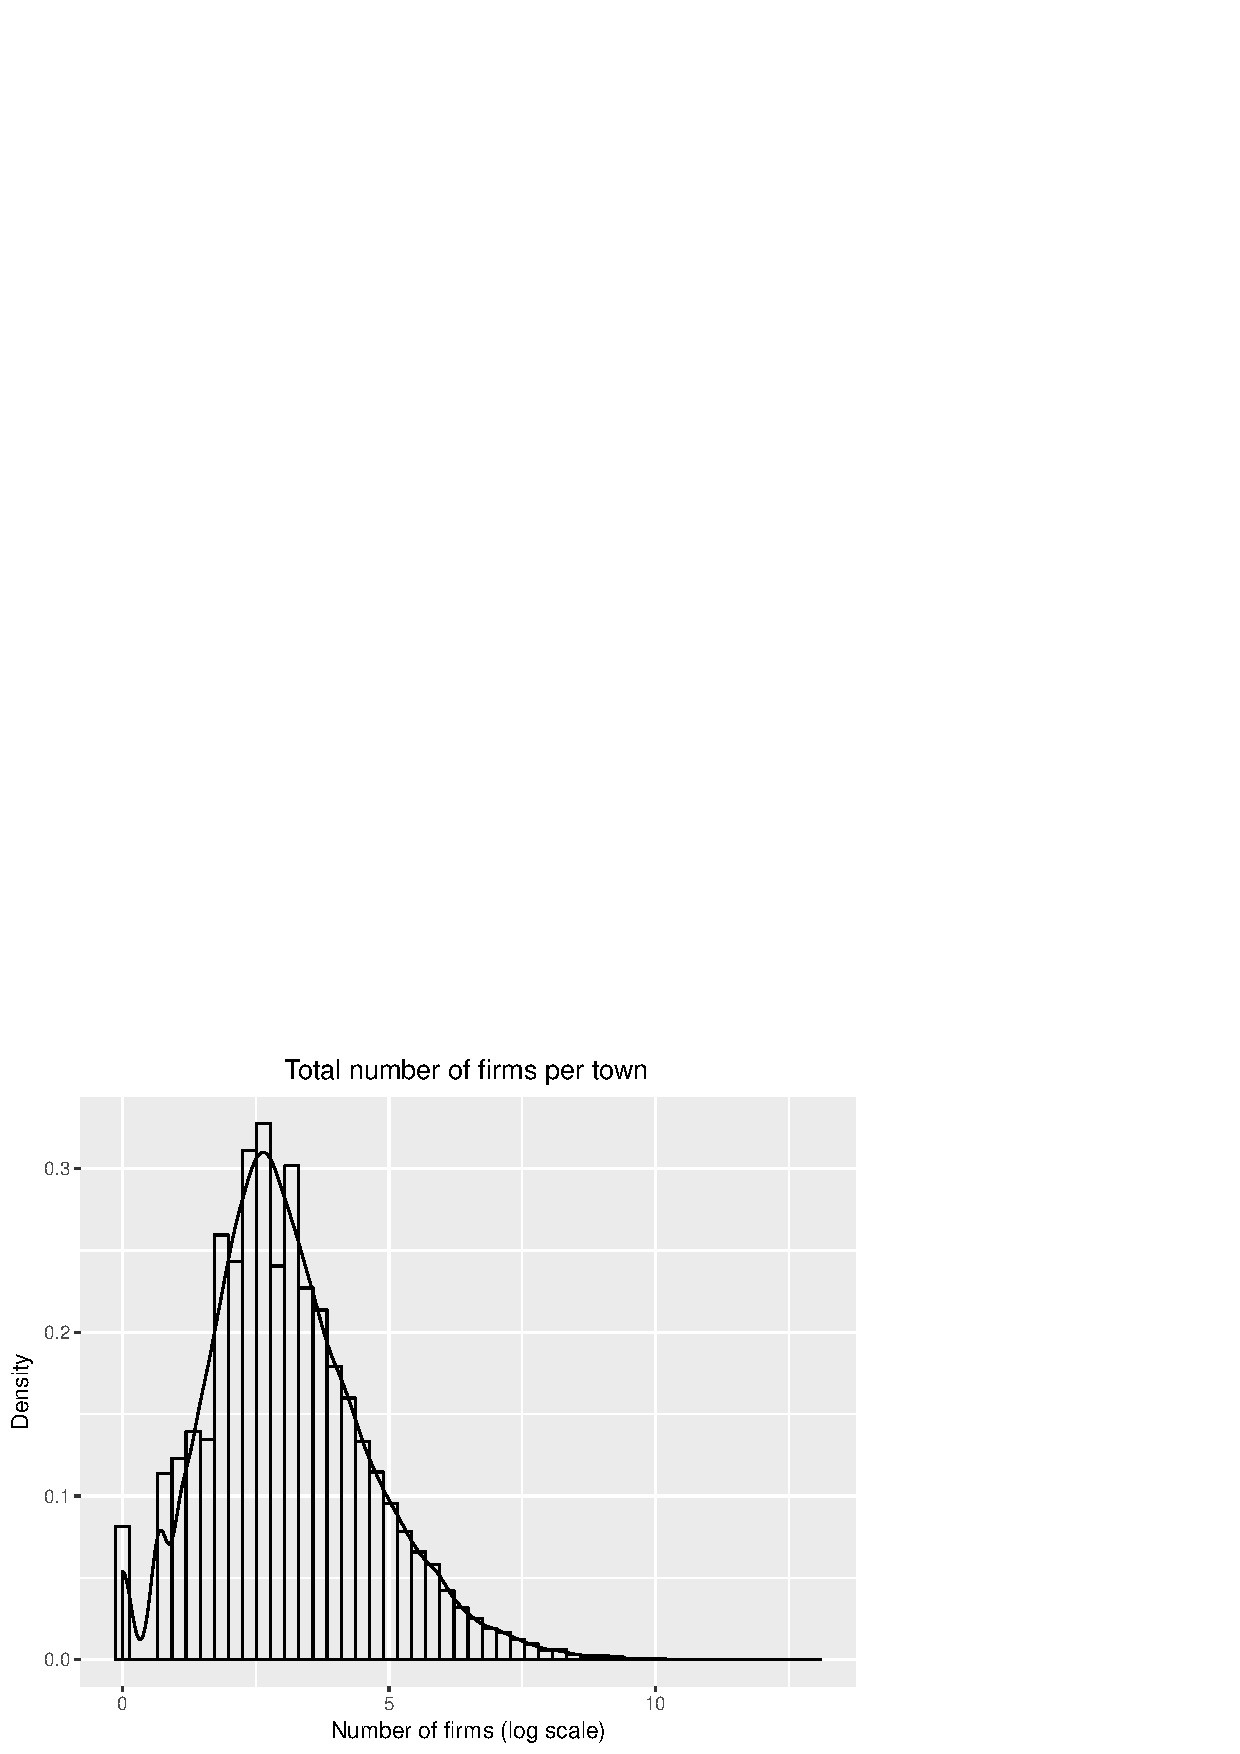
\includegraphics[width=0.5\textwidth]{hist_firms_total.jpeg}}
				\subfloat{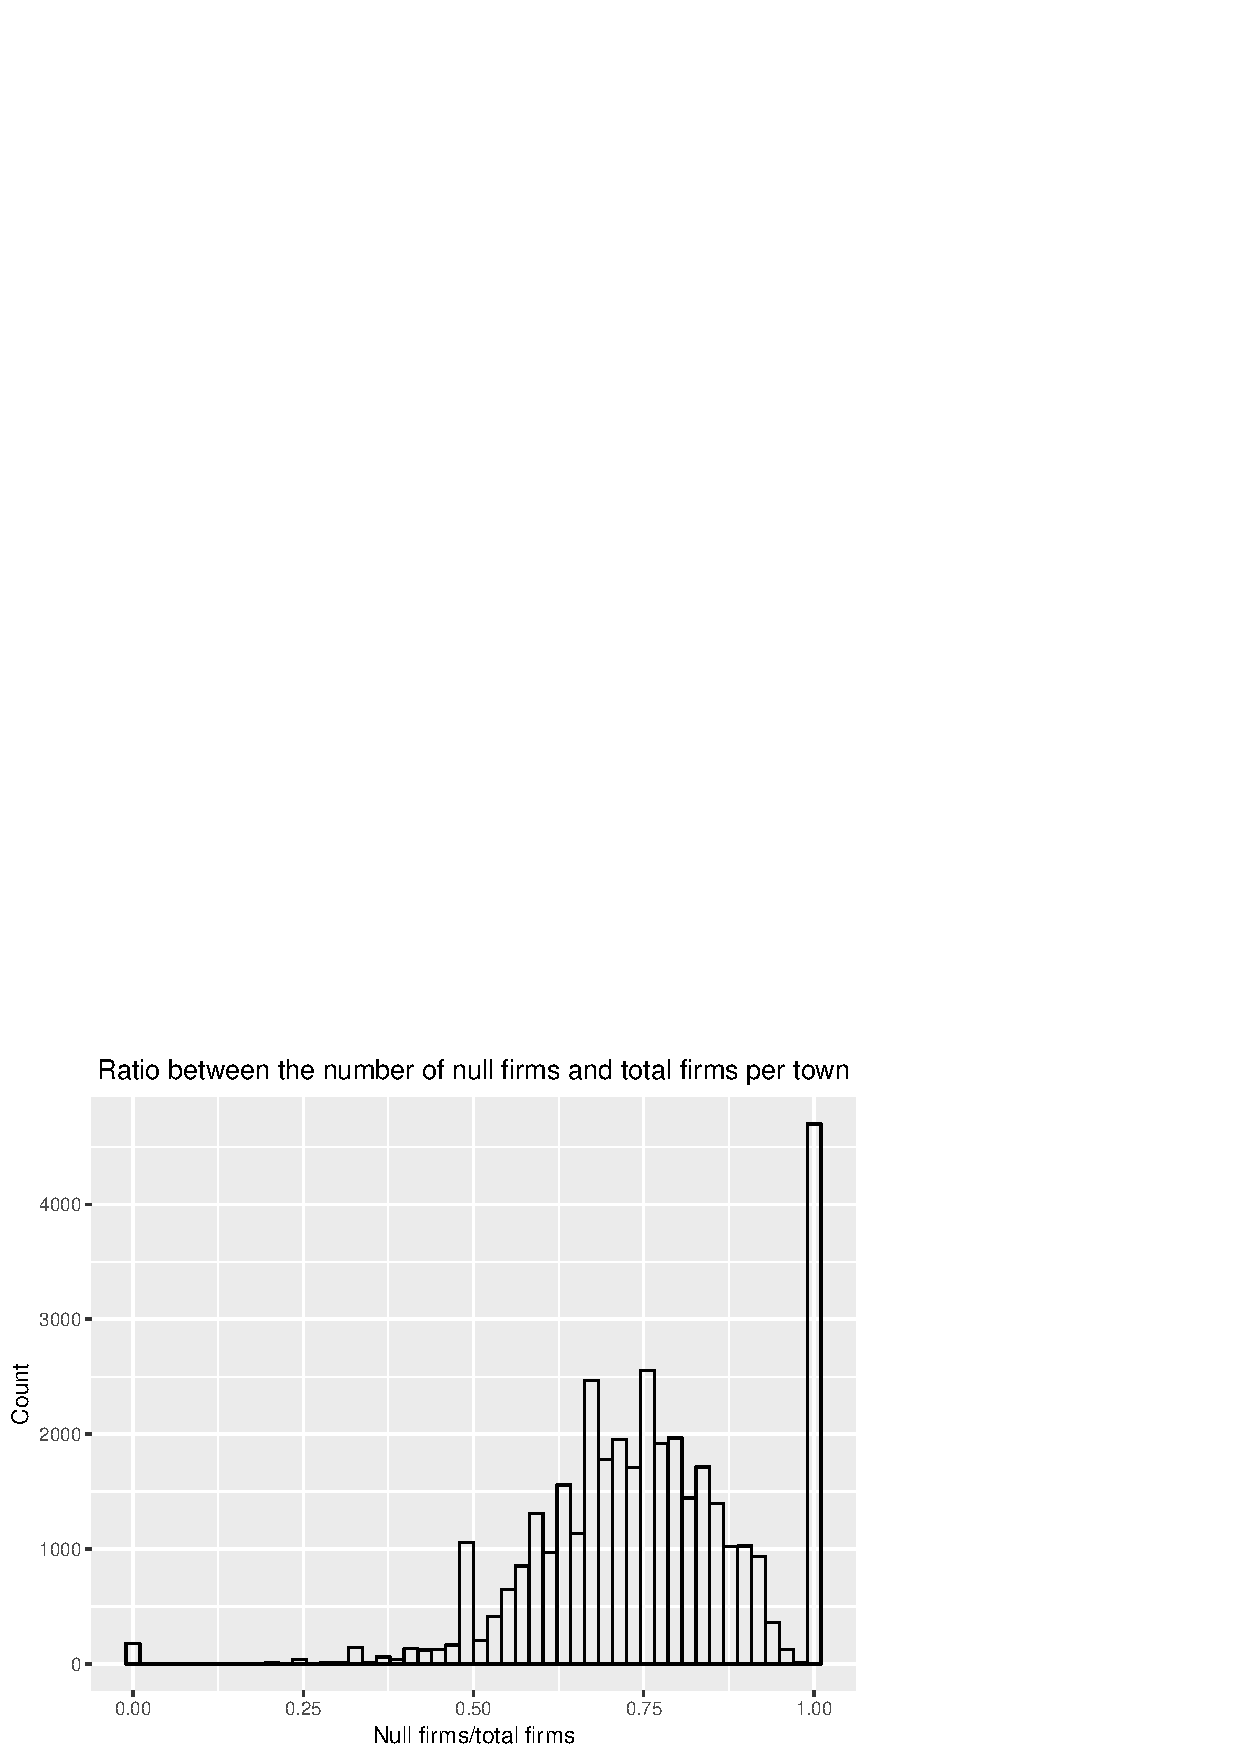
\includegraphics[width=0.5\textwidth]{hist_firms_ratio_null_total.jpeg}}
%				\caption{} 
%				\label{}
			\end{figure}
\end{frame}


\section{3.1 Graphes}
\begin{frame}{\centerline{\huge\textcolor{bscuro}{Firms}}}
%Fig.~\ref{fig4} shows 
	\begin{itemize}
		\item PCA analysis
	\end{itemize}

\begin{figure}[!ht] 
	\centering
	\subfloat{\includegraphics[width=0.7\textwidth]{biplot_firms.jpeg}}
%	\subfloat[]{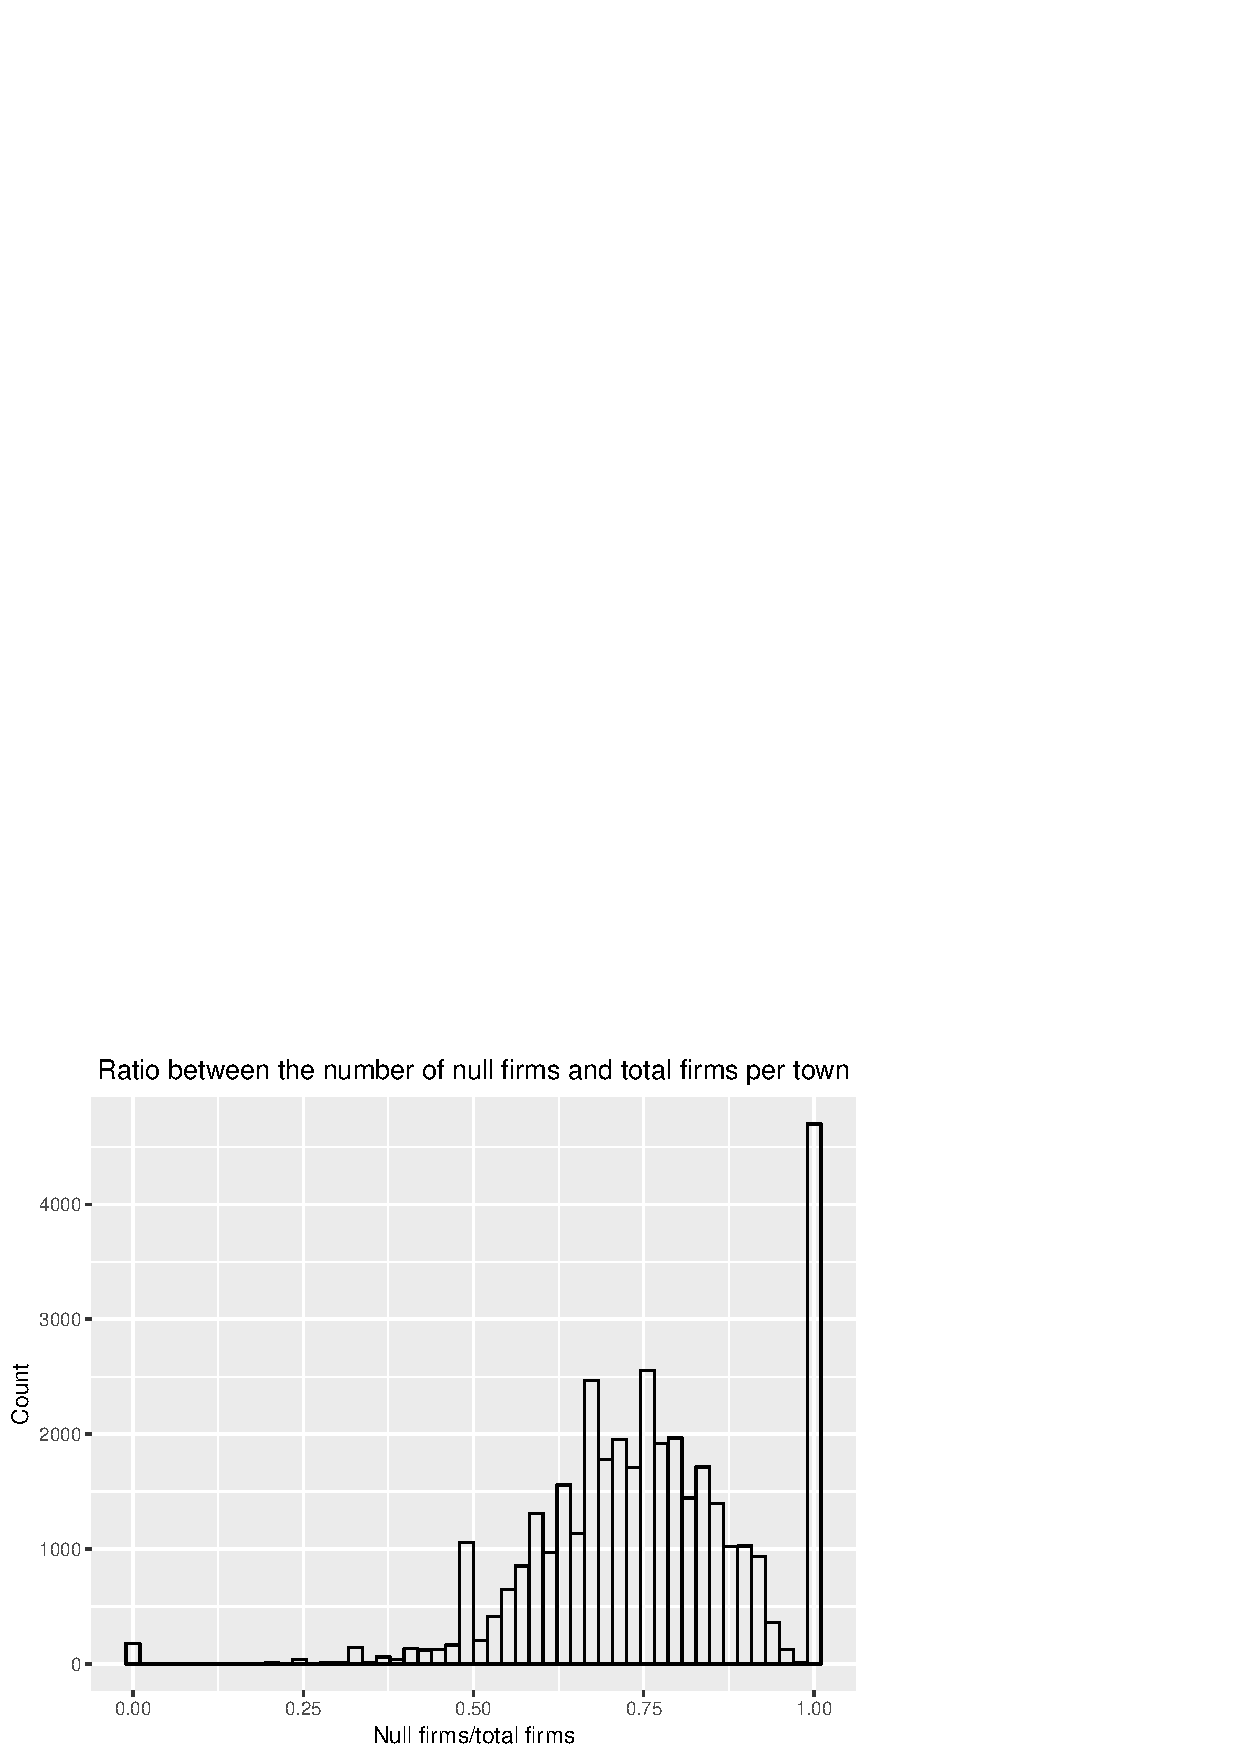
\includegraphics[width=0.5\textwidth]{hist_firms_ratio_null_total.jpeg}}
%	\caption{} 
%	\label{fig4}
\end{figure}
\end{frame}


%\section{4. What has been done so far...}
%	\begin{frame}{\centerline{\huge\textcolor{bscuro}{Geography}}}
%		\begin{itemize}
%			\begin{itemize}
%				\item xx;
%		\end{itemize}
%\end{frame}


\section{Issues}
		\begin{frame}{\vskip 0.05cm\centerline{\Huge\textcolor{bscuro}{Issues}}}
		
				\begin{itemize}
						\item A lot of NA in geo locations (retrieved from Google API)
						\item Unique code for salary data 1/7 of the total 
						\item Missing additional information 
						\item French DOM-TOM regions
						\item Outliers and spatial correlation
				\end{itemize}

\end{frame}			
		

\section{Future works}
		\begin{frame}{\vskip 0.05cm\centerline{\Huge\textcolor{bscuro}{Future works}}}
%		Elaborate on future plans; can what you did during the course be the basis for a continuing project/collaboration? 

\begin{itemize}
	\item Combine the separated datasets
	\item Create meaningful indicators
	\item Take correlation into account (especially spatial)
	\item Perform clustering techniques to identify geographical clusters
	\item Perform groupwise lasso to predict salary data
	\item Verification/improvement of the obtained results 
	\item Compare the methodologies used with robust ones
	\item Find complementary datasets
\end{itemize}

\end{frame}		
	
\section{End}
	\begin{frame}
	\centerline{\Huge\textcolor{bscuro}{ -- \emph{Thank you} -- }}
\end{frame}

\end{document}
